\section{Laboratory work implementation}

\subsection{Tasks and Points}

\begin{itemize}
	\item Basic Level (nota 5 || 6):
	
	\begin{itemize}
		\item Realizeaza un simplu GUI calculator care suporta functiile de baza: +, -, /, *.
	\end{itemize}
	
	\item Normal Level (nota 7 || 8):
	
	\begin{itemize}
		\item Realizeaza un simplu GUI calculator care suporta urmatoare functii: +, -, /, *, putere, radical, InversareSemn(+/-).
	\end{itemize}
	\item Advanced Level (nota 9 || 10):
	
	\begin{itemize}
		\item Realizeaza un simplu GUI calculator care suporta urmatoare functii: +, -, /, *, putere, radical, InversareSemn(+/-), operatii cu numere zecimale.
	\end{itemize}
	\begin{itemize}
		\item Divizare proiectului in doua module - Interfata grafica(Modul GUI) si Modulul de baza(Core Module).
	\end{itemize}
\end{itemize}
\subsection{Analiza lucrarii de laborator}

Link SSH la repozitoriu: git@github.com:croitoruion/MIDPS.git


Am realizat un simplu calculator in IDE-ul Visual Studio 2010 in limbajul Csharp.

\begin{center}
	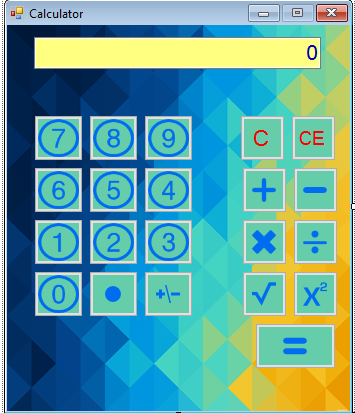
\includegraphics[width=0.7\linewidth]{../../screenshots/calculator}
\end{center}
Calculatorul dat poate realiza urmatoarele functii: Adunarea,scaderea,impartirea,inmultirea,inversarea semnului,ridiare la putere,radical.Totodata toate aceste functii pot fi aplicare numerelor cu virgula.

Visual Studio ne propune o paleta larga de instrumente unde putem gasi toate cele necesare pentru crearea a unor aplicatii simple

\begin{center}
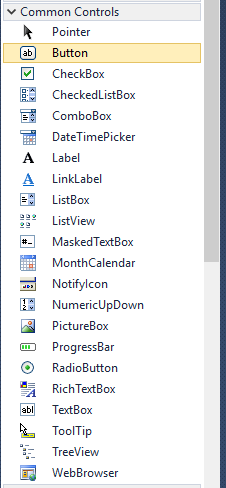
\includegraphics[width=0.7\linewidth]{../../screenshots/toolbox}
\end{center}

Aici putem selecta ce avem nevoie,de exemplu in programul meu am folosti Butoane pentru cifre si operatii si textBox-ul afisarea cifrelor introduse si rezultatul in urma efectuarii operatiilor

Cand selectam un buton sau oricare alt obiect din programul nostru observam ca apare in partea dreapta un Dialog-Box cu proprietati unde putem edita obiectul nostru.De exemplu daca este button putem sa-i atribuim un text ,care se va afisa pe button,putem edita acest text in toate modalitatile (fonturi/culori/dimensiuni s.a.)
putem alege un background solid color sau o imagine oricare dorita
\begin{center}
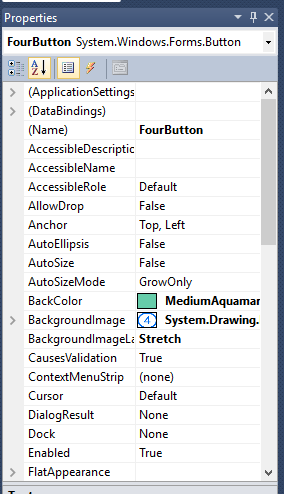
\includegraphics[width=0.7\linewidth]{../../screenshots/prop}
\end{center}

De la inceput am utilizat cifre pentru butoane si totodata toate functiile cu aceste butoane erau carcaterizate de cimpul text,astfel cand se apela functia DigitClick functia cauta valoarea text-ului buttonului si o utiliza drept variabila.

\begin{center}
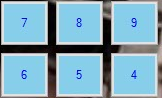
\includegraphics[width=0.7\linewidth]{../../screenshots/cifre1}
\end{center}


\begin{center}
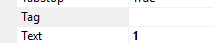
\includegraphics[width=0.7\linewidth]{../../screenshots/text}
\end{center}

Mai apoi am utilizat icons in loc de cifre pe buttoane,icon-urile reprezinta nu altceva decat un background imagine bitmap pe fundalul acestui button.Astfel trebuia de sters textul pe button si de atribuit la Tag aceasta valoare,insa a fost nevoita schimbarea a tuturor functiilor legate de acest button.In final 

\begin{center}
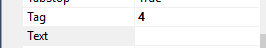
\includegraphics[width=0.7\linewidth]{../../screenshots/tag}
\end{center}

\begin{center}
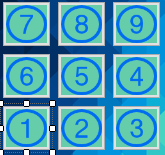
\includegraphics[width=0.7\linewidth]{../../screenshots/cifre}
\end{center}
La fel am gasit si am importat bitmapuri pentru toate butoanele utilizate.


Am implementat o functie universala pentru toate butoane-cifre de introducerea valorii.Aceasta a optimizat un pic codul programului
\begin{center}
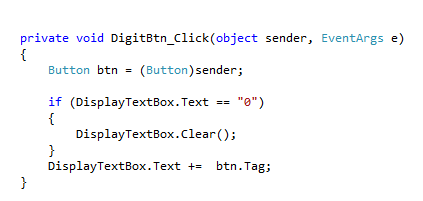
\includegraphics[width=0.7\linewidth]{../../screenshots/buttonClick}
\end{center}

Pentru efectuarea operatiilor a fost nevoie de cateva variabile globare
\begin{center}
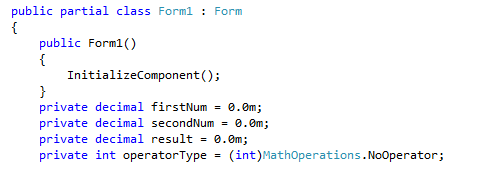
\includegraphics[width=0.7\linewidth]{../../screenshots/varglobale}
\end{center}
Toate operatiile inafara de radical se efectuaeaza odata cu apasarea butonului = .Efectuarea operatiilor are loc conform urmatorului algoritm:Scrim 1 cifra(salvam in var globala) apoi alegem operatia salvam variabila operatiei,introducem a 2 cifra(salvam a 2 var globala),apoi la apasarea butonul = functia citeste variabila operatiiei si alege case-ul potrivit si efectueaza operatia afisind rezultatul in DIsplayBox
\begin{center}
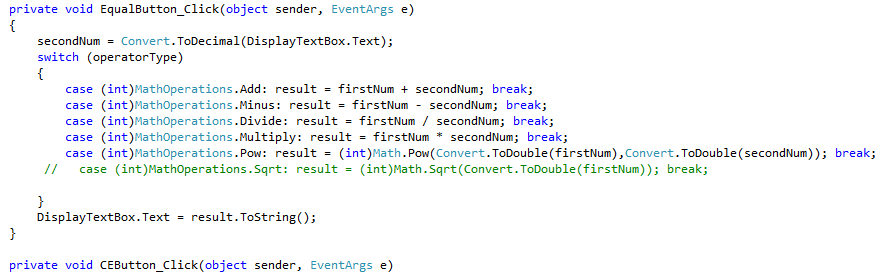
\includegraphics[width=0.7\linewidth]{../../screenshots/EqualB}
\end{center}

Implementarea butoanelor C si CE.
La apasarea butonului CE se egaleaza cu 0 valoarea curenta a textBoxului.
La apasarea butonului C se egaleaza cu 0 toate variabile globale utilizate 
\begin{center}
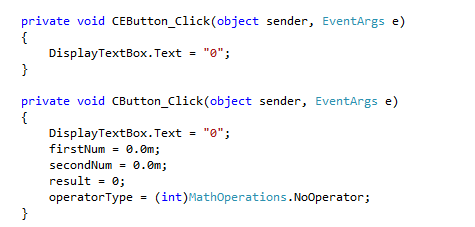
\includegraphics[width=0.7\linewidth]{../../screenshots/C_CE}
\end{center}

